%%%% ijcai16.tex

\typeout{IJCAI-16 Instructions for Authors}

% These are the instructions for authors for IJCAI-16.
% They are the same as the ones for IJCAI-11 with superficical wording
%   changes only.

\documentclass{article}
% The file ijcai16.sty is the style file for IJCAI-16 (same as ijcai07.sty).
\usepackage{ijcai16}
\usepackage{algorithm}
\usepackage{algpseudocode}

\usepackage{graphicx}

\usepackage{verbatim}
\usepackage{amssymb}
\usepackage{amsmath}

\usepackage{enumitem}

\usepackage{setspace}
% Use the postscript times font!
\usepackage{times}

% the following package is optional:
%\usepackage{latexsym}


\title{Ultra-sensitive variant detection with improved accuracy using variational inference for heterogeneous next-generation sequencing data}

\author{Fan Zhang \\
Worcester Polythechnic Institute, MA  \\
fzhang@wpi.edu}

\begin{document}

\maketitle

\begin{abstract}
We propose a variational inference algorithm to estimate variant allele frequency (VAF) and identify single nucleotide variants in heterogeneous next-generation sequencing data.
We demonstrate our variational algorithm with higher sensitivity and specificity than Markov Chain Monte Carlo (MCMC) sampling method on a synthetic data set,
and more efficient at relative low median read depths of 10x and 100x.
We apply our algorithm on a longitudinal anti-cancer drug resistance sequencing data set and identify XXX variants that XXX.
We also show that our model with variational algorithm has an improved performance in XXX on a longitudinal clinical data set compared with the state of arts approaches.
\end{abstract}

\section{Introduction}
Next-generation sequencing (NGS) data and single nucleotide variants (SNVs).
xxx\\
xxx\\
xxx\\
xxx\\
xxx\\
xxx\\
xxx\\
xxx\\

Variants detection methods and problems.
xxx\\
xxx\\
xxx\\
xxx\\
xxx\\
xxx\\
xxx\\
xxx\\

Recently, some algorithms have been developed Bayesian models to identify SNVs in NGS data.
The main computational problem for probabilistic Bayesian models is posterior inference.
There are two popular ways to do posterior inference- Markov Chain Monte Carlo (MCMC) samplings, and variational algorithms.
MCMC is a simple algorithm for sampling, which is easy to understand. The main problem of MCMC is that it is hard to diagnose convergence and handle nonconjugate events.
The main idea of variational inference is propose a variational distribution over latent variables and optimize the variational parameters to make the proposal distribution close to the true posterior distribution. 
So variational inference is more accurate to handle nonconjugate distirbutions and more efficient than MCMC. 
RVD2 uses a hierarchical Bayesian model to estimate allele frequency and call variants by deriving a Metropolis-within-Gibbs sampling inference algorithm [cite RVD2].
Generally speaking, this algorithm is able to accurately estimate variant allele frequencies (VAFs), but it shows a relatively low specificity when the variant allele frequency is low (less than 1.0$\%$) but the median read depth is very high (40000x).


We show that we develop a variational expectation-maximization (EM) algorithm for our Bayesian statistical model to achieve sufficient accuracy and efficiency to identify variants in heterogeneous call samples. First, our variational EM algorithm is able to accurately approximate the posterior distribution of latent variables for a pair of samples- the sample of interest and a known reference sample. Then, a hypothesis test calls a variant by a significant difference between the key model parameters of this pair of samples. We compare the performance of variational inference algorithm to MCMC sampling method and several other variant detection methods. Finally, we demonstrate our variational algorithm on a longitudinal time-series DNA sequencing data to quantify the degree to which the variant modulates resistance to anti-cancer drug.

\section{Model Structure}
Our Bayesian statistical model is shown as a graphical representation in Figure~\ref{tbl:graphical_model}. $r_{ji}$ is the number of reads with a non-reference base at location $j$ in experimental replicate $i$. $n_{ji}$ is the total number of reads at location $j$ in experimental replicate $i$. 
\begin{figure}[htpb]
\centering
\vspace{-10pt}
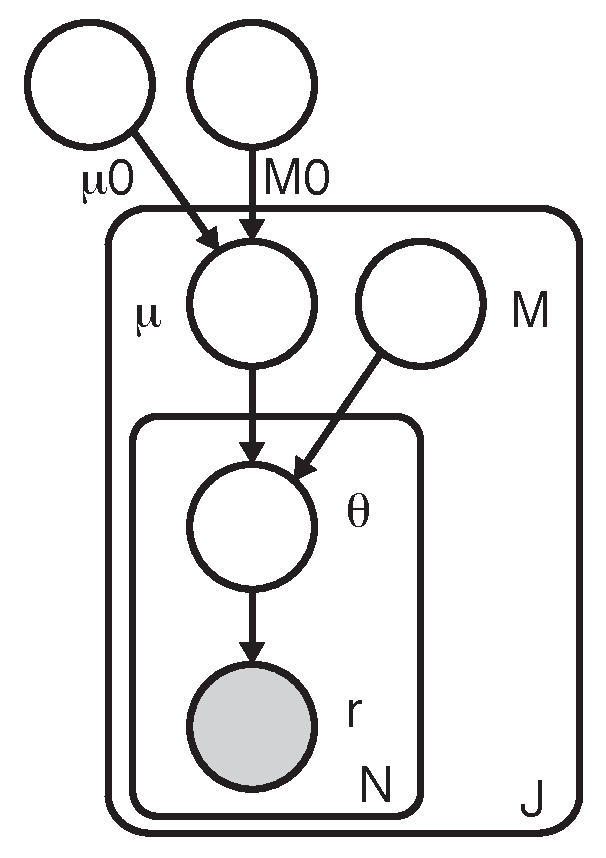
\includegraphics[width=0.18\textwidth]{figs/RVD3_model.pdf}
\caption{Graphical model representation of our Bayesian model.
$\mu_0$, a global error rate; $M_0$, a global precision;  $ \mu_j $, a local error rate. $M_j$, a local precision. $\mu_0$, a global error rate to estimate the expected error rate across all locations. $M_0$, a global precision, estimates the variation in the error rate  across locations. The local error rate, $ \mu_j $, estimates the exepected error rate across replicates at location $ j $. The local precision, $M_j$, estimates the variation in the error rate across replicates at location $j$}
\label{tbl:graphical_model}
\end{figure}
The model generative process is as follows:
\begin{enumerate}[noitemsep]
	\item For each location $j$:
	\begin{enumerate}
		\item Draw an error rate $\mu_j \thicksim \text{Beta}(\mu_0, M_0)$
		\item For each replicate $i$:
		\begin{enumerate}
			\item Draw $\theta_{ji} \thicksim \text{Beta}(\mu_j, M_j)$
			\item Draw $r_{ji} | n_{ji} \thicksim \text{Binomial}(\theta_{ji}, n_{ji})$
		\end{enumerate}
	\end{enumerate}
\end{enumerate}


\section{Inference and Hypothesis Testing}
\subsection{Variational Expectation Maximization (EM) Inference}
RVD3 improves RVD2 in the way of posterior distribution inference. We develop a non-conjugate variational inference algorithm to approximate the posterior distrubtion, 
\begin{equation}
	p(\mu, \theta | r, n; \phi)  = \frac{ p(\mu, \theta, r | n; \phi) } {p ( r | n; \phi)},
\end{equation}
where the parameters are $\phi \triangleq \{\mu_0, M_0, M\}$.
\subsubsection{Factorization}
We propose the following factorized variational distribution to approximate the true posterior over latent variables $\mu_j$ and $\theta_{ij}$. $q(\mu_j)$ approximates the variational posterior distribution of $\mu_j$, which represents the local error rate distribution in position $j$ across different replicates.
$q(\theta_{ij})$ approximates the posterior distribution of $\theta_{ij}$, which is the error rate distribution in position $j$ replicate $i$.
\begin{equation}
  q(\mu, \theta) = q(\mu)q(\theta) = \prod_{j=1}^J q(\mu_{j}) \prod_{i=1}^N q(\theta_{ji}).
  \label{eq:vardist}
\end{equation}

\subsubsection{Evidence Lower Bound (ELBO)}
The log-likelihood of the data is lower-bounded according to Jensen's inequality:
\begin{equation}
\begin{split}
\log p \left( r | \phi \right) &= \log \int_\mu \int_\theta p\left(r,\mu,\theta \right) d\theta d\mu \\
&= \log \int_\mu \int_\theta p\left(r,\mu,\theta \right)\frac{q\left(\mu,\theta \right) }{q\left(\mu,\theta \right) } d\theta d\mu \\
&\geq \int_\mu \int_\theta q\left(\mu,\theta \right) \log \frac{ p\left(r,\mu,\theta \right)}{q\left(\mu,\theta \right)} d\theta d\mu \\
&= E_q \left[ \log p\left(r,\mu,\theta \right)\right] - E_q \left[ \log q\left(\mu,\theta \right)\right] \\
&\triangleq \mathcal{L}(q, \phi).
\end{split}
\end{equation}
where $ \phi= \left( \mu_0, M_0, M \right) $.

The item $\mathcal{L}(q, \phi)$ is the evidence of lower bound (ELBO) of the log-likelihood of the data, which is the sum of $q$-expected complete log-likelihood and the entropy of the variational distribution $q$.
The goal of variational inference is maximizing the ELBO.
Equivalently, $q$ is chosen by minimizing the Kullback-Liebler (KL) divergence between the variational distribution and the true posterior distribution.

\subsubsection{Variational Distributions}
The posterior distribution of $\theta_{ij}$ is a Beta distribution,
\begin{align}
&p(\theta_{ji}|r_{ji},n_{ji},\mu_j,M_j)\\
&\thicksim \text{Beta}(r_{ji}+M_j \mu_j, n_{ji}-r_{ji}+M_j(1-\mu_j)).
\end{align}
Therefore, we propose Beta distribution with parameter vector $\delta_{ji}$ as variational distribution,
\begin{align}
\theta_{ji} &\thicksim \text{Beta}(\delta_{ji}) \nonumber
\end{align}
%
The posterior distribution of $\mu_j$ is given by its Markov blanket
\begin{align}
p(\mu_j|\theta_{ji},M_j,\mu_0,M_0)\propto p(\mu_j|\mu_0,M_0)p(\theta_{ji}|\mu_j,M_j).
\end{align}
This is not in the form of any known distribution. Therefore, we propose Beta distribution with parameter vector $\gamma_{ji}$ as variational distribution to simplify the variational derivation.
\begin{align}
\mu_j &\thicksim \text{Beta}(\gamma_j) \nonumber
\end{align}

\subsubsection{Variational Expectation Maximization (EM) Algorithm}
Variational EM maximizes the ELBO on the true likelihood, by alternating between maximization over $q$ (E-step) and maximization over $\phi$ (M-step).

\begin{algorithm}[h]
  \caption{RVD3 Variational Inference}

  \begin{algorithmic}[1]

  \State Initialize $ q(\theta, \mu) $ and $\hat{\phi}$

  \Repeat

	\Repeat
	
		\For {j = 1 to J}					
			\For {i = 1 to N}				
			\State Optimize $\mathcal{L}(q, \hat{\phi})$ over $q(\theta_{ji}; \delta_{ji}) = \text{Beta} (\delta_{ji})$				
			\EndFor			
		\EndFor
	
		\For {j = 1 to J} 		
			\State Optimize $\mathcal{L}(q, \hat{\phi})$ over $q(\mu_j; \gamma_j) = \text{Beta} (\gamma_j)$			
		\EndFor
	
	\Until{change in $\mathcal{L}(q,\hat{\phi})$ is small}

  \State Set $\hat{\phi} \leftarrow \arg \max\limits_{\phi}
            \mathcal{L}(q,\phi)$
  \Until {change in $\mathcal{L}(q,\hat{\phi})$ is small}

  \end{algorithmic}

\end{algorithm}

\section{Posterior Distribution Test}
\subsection{Z-test for Gaussian Distribution}
Variational inference provides variational distributions for $q(\mu_j|r^{control})$ and $q(\mu_j|r^{case})$, which are approximated to the posterior distributions for $p(\mu_j|r^{control})$ and $p(\mu_j|r^{case})$.
We use $Z$-test based on Gaussian distribution.
%\begin{equation}
\begin{align}
\label{eq:test}
& \mu_j^{\triangle} = \mu_j|r^{case}-\mu_j|r^{control}\\
& \sigma_j^{\triangle} = \sqrt {var_q{[\mu_j|r^{case}]} + var_q{[\mu_j|r^{control}]}}\\
& Z_j = \frac{\tau - \mu_j^{\triangle}}{{\sigma_j}^{\triangle}}\\
& Pr(Z_j) < \alpha
\end{align}
%\end{equation}
where $\tau$ is a detection threshold and $\alpha$ is a significance level. Here we set $\tau = 0$ and $\alpha = 0.05$.
$\mu_j^{case}$ and $\mu_j^{control}$ are means of distributions.
$var_q{[\mu_j|r^{case}]}$ and  $var_q{[\mu_j|r^{control}]} $are variances of distributions.
A position is called as a variant when the p-value is less than the significant level $\alpha$.

$\chi^2$ goodness-of-fit test for non-uniform base distribution is also used to distinguish a scenario of a true variant from a scenario of a random seuqencing error [cite RVD2]. 

%\subsection{Posterior Odds Ratio}

\section{Data Sets}
\subsection{Synthetic DNA Sequence Data}
We synthesized two random 400bp DNA dequences. One sample with 14 loci variants is taken as the case and the other without variants is taken as the control.
Case and control samples were mixed to yield defined VAFs of $0.1\%$, $0.3\%$, $1.0\%$, $10.0\%$, and $100.0\%$.
The details of the experimental protocal are available in [cite RVD].
The synthetic DNA data were downsampled by 10x, 100x, 1,000x, and 10,000x using Picard.
The final data set contains read pairs for 6 replicates for the control at different VAF levels.

\subsection{Longitudinal Drug Resistance Data}
xxx\\
xxx\\
xxx\\
xxx\\
xxx\\
xxx\\
xxx\\
xxx\\
xxx\\
xxx\\
xxx\\
xxx\\

%\subsection{Longitudinal Directed Evolution Data}

\section{Results}
\subsection{Performance on Synthetic DNA Data}
\subsubsection{Comparison of Sensitivity and Specificity}
The posterior distribution over latent variables can be inferenced using either MCMC sampling method or variational algorithm.
We compare the performance of variational algorithm and MCMC sampling method in the performance of sensitivity and specificity (Figure~\ref{tbl:statistics_mcmc_var}).
We use posterior distribution test with $\chi^2$ test to detect variants for a broad range of median read depths and different variant allele frequencies (VAFs).
Variational algorithm works best compared with MCMC in sensitivity and specificity.
The converging process for estimating variational posterior for VAF=$100.0\%$ at median read depth of 30590x is shown in (Figure~\ref{tbl:converge_ELBO.png}). It takes 60 variational EM iterations to stop converging when the increased ELBO rate is less than $0.1\%$. 

%The specificity is getting a little worse when the median read depth increases from $4000X$ to $400000X$ in the events of $VAF=0.1\%$, $0.3\%$, and $1.0\%$.
%The specificity is improved when tightening the stop criterion of ELBO update from $1.0\%$ to $0.1\%$.

%The specificity could be not ideal if the chosen initial values lead the variational distribution to a local optimum, which could be happened in the variational approximation algorithm. We can consider about randomly testing different initial values for $\delta$ and $\gamma$ to get rid of the local optimums results. %Threshold for $\delta$ update and $\gamma$ update is also set to guarantee its update.

% results are under folder \fzhang\Research\rvd3-variational-notebook\results\2015-09-28_Run_rvd3_synthetic_data_set
\begin{table}[h]
\centering
\vspace{-5pt}
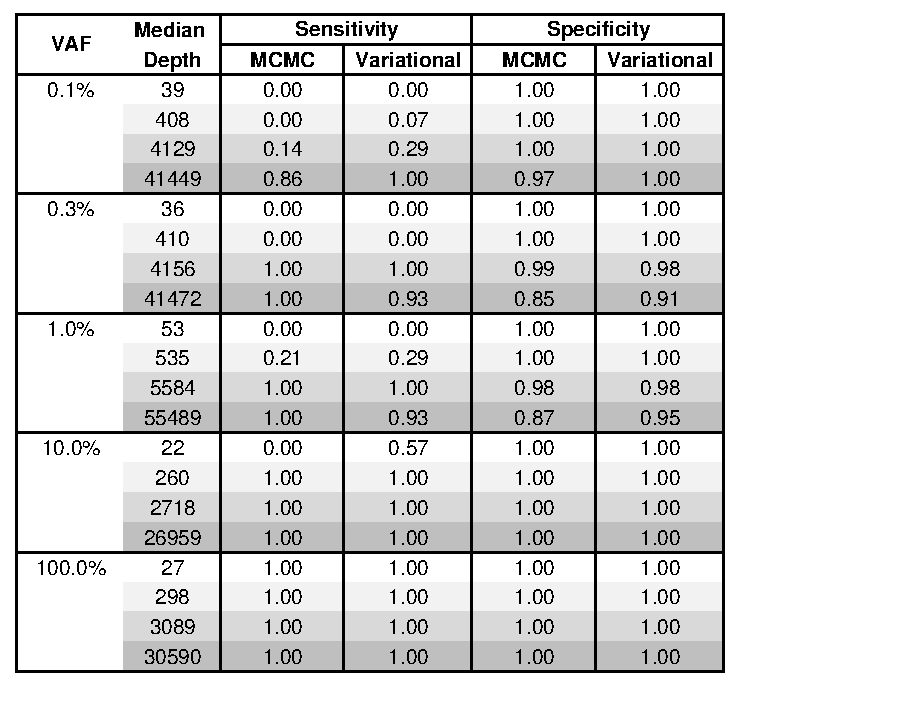
\includegraphics[width=0.6\textwidth]{tables/statistics_mcmc_var.pdf}
\caption{Sensitivity/Specificity comparison of variational algorithm with MCMC on the synthetic DNA data set.}
\vspace{-10pt}
\label{tbl:statistics_mcmc_var}
\end{table}

% results are under folder \fzhang\Research\rvd3-variational-notebook\results\2015-11-05_Plot_ELBO_rvd3
\begin{figure}[h]
\centering
\vspace{-5pt}
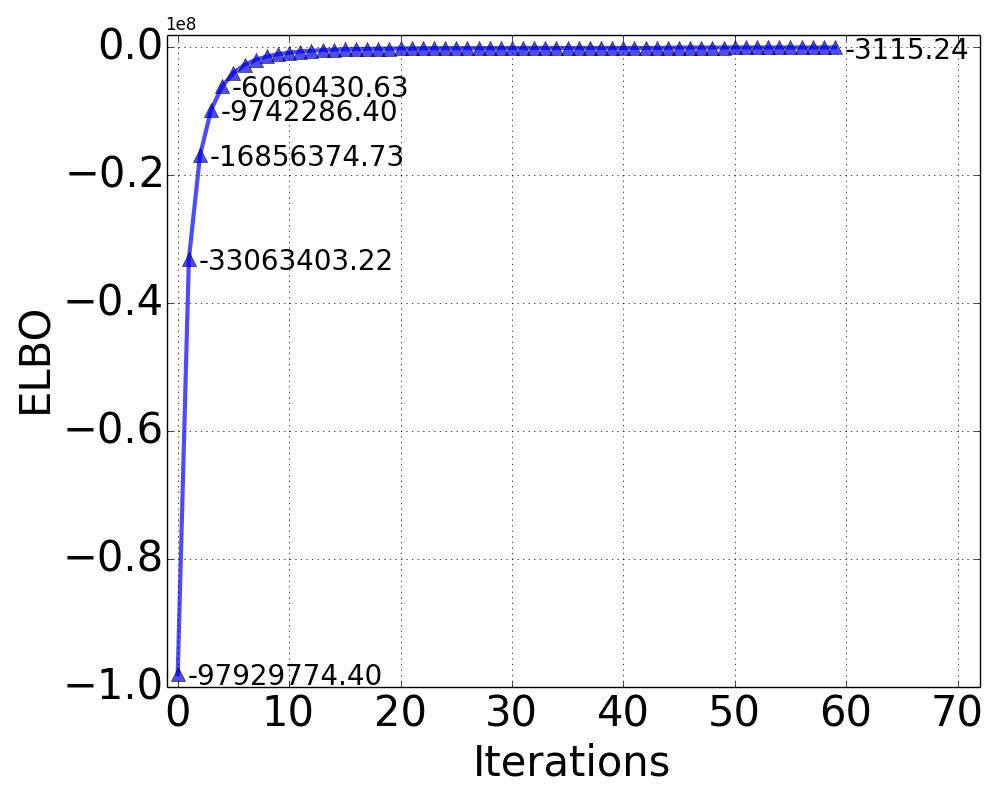
\includegraphics[width=0.45\textwidth]{figs/converge_ELBO.png}
\caption{Converging ELBO for estimating variational posterior in the event of VAF=$100.0\%$ at median read depth of 30590x.}
\vspace{-10pt}
\label{tbl:converge_ELBO.png}
\end{figure}


\subsubsection{Comparison of Approximated Posterior Distribution}
We show the approximated posterior distribution of variational algorithm and exact samples of MCMC.
A true variant position 85 of sample of VAF=$1.0\%$ is taken as an example.
Variational and MCMC both identify this position at median read depth of 5584 (Figure~\ref{tbl:combine_posterior}).
The specificity of variational is higher than MCMC at the highest median read depth when VAF is $0.1\%$, $0.3\%$, and $1.0\%$ , which shows that MCMC calls more false positive positions.
Here we show the approximated distribution of a false positive position 144 identified by MCMC, while it is not identified by variational algorithm (Figure~\ref{tbl:posterior_mcmc_var_3}).
Here the variance of variational distributions is wider than that of MCMC sampling, which makes the difference of these two distributions are not significant enough to be called as a variant by variational algorithm. 
It shows that variational algorithm gives a deterministic approximation of posterior distribution that is more accurate than stochastic sampling does.
It is also noticeable that the shape of variational distributions using Beta distribution is very close to Gaussian distribution.

% results are under folder \fzhang\Research\rvd3-variational-notebook\results\2015-10-14_Plot_mcmc_mu_vs_variational_mu
\begin{figure}[h]
\centering
\vspace{-10pt}
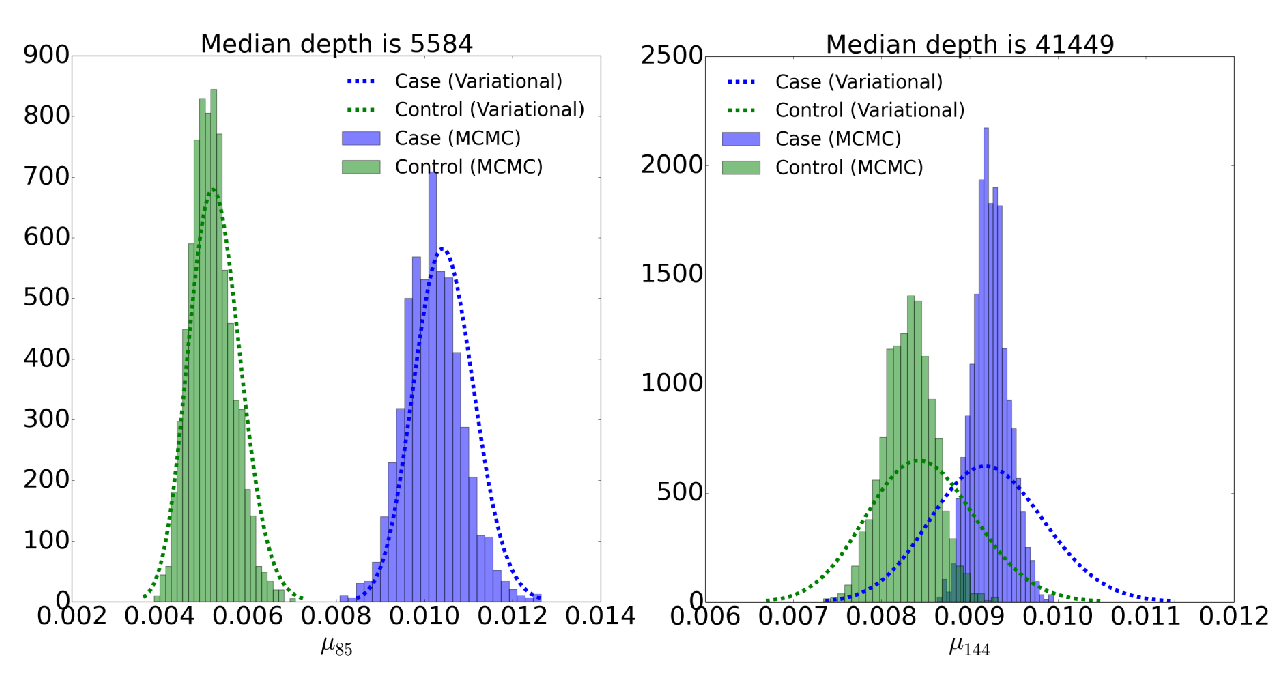
\includegraphics[width=0.5\textwidth]{figs/combine_posterior.pdf}
\caption{Approximated posterior distribution by variational algorithm and MCMC. Position 85 when median read depth is 5584 is a true variant. Position 144 when median read depth is 41449 is a false positive position that is identified by MCMC, while variational algorithm does not identify this as a variant.}
\vspace{-5pt}
\label{tbl:combine_posterior}
\end{figure}

%\begin{figure}[h]
%\centering
%\vspace{-10pt}
%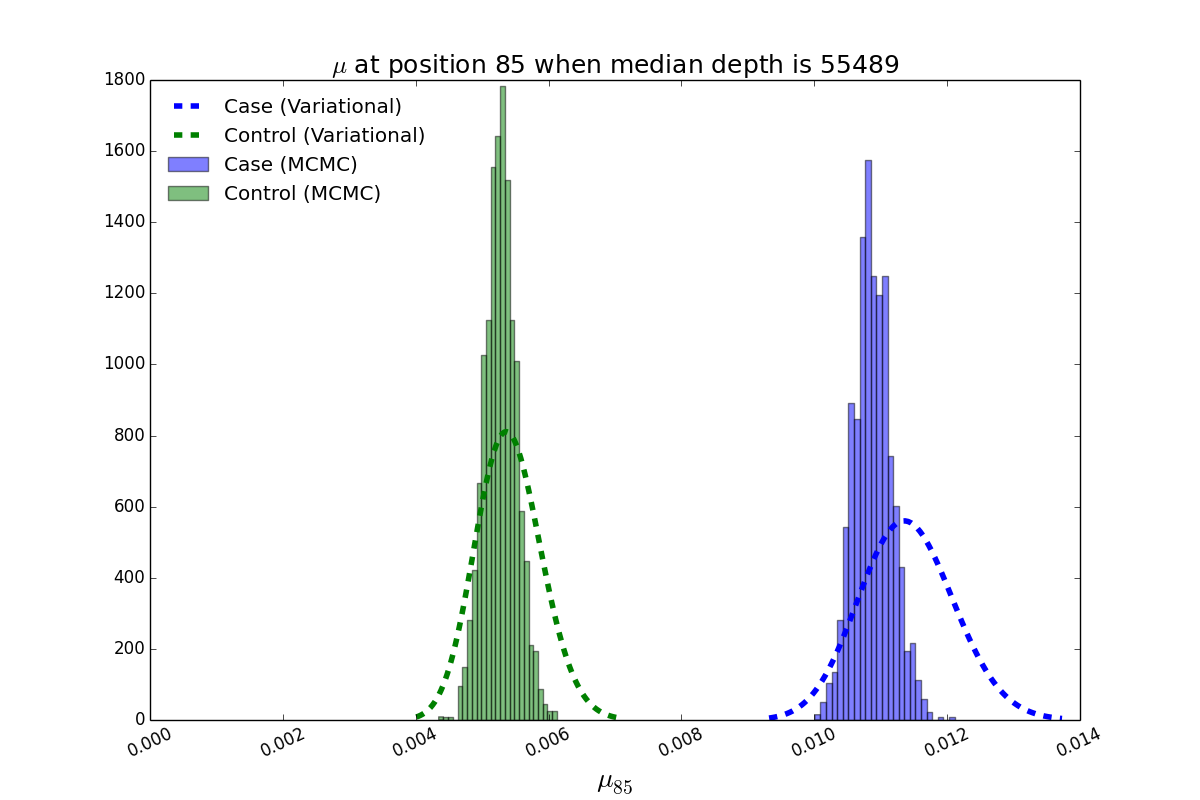
\includegraphics[width=0.5\textwidth]{figs/position_85_55489_mcmc_vs_var_mu.png}
%\caption{Approximated posterior distribution by variational algorithm and MCMC for position 85 when median read depth is 55489.}
%\vspace{-10pt}
%\label{tbl:posterior_mcmc_var_2}
%\end{figure}

%\begin{figure}[!htbp]
%\centering
%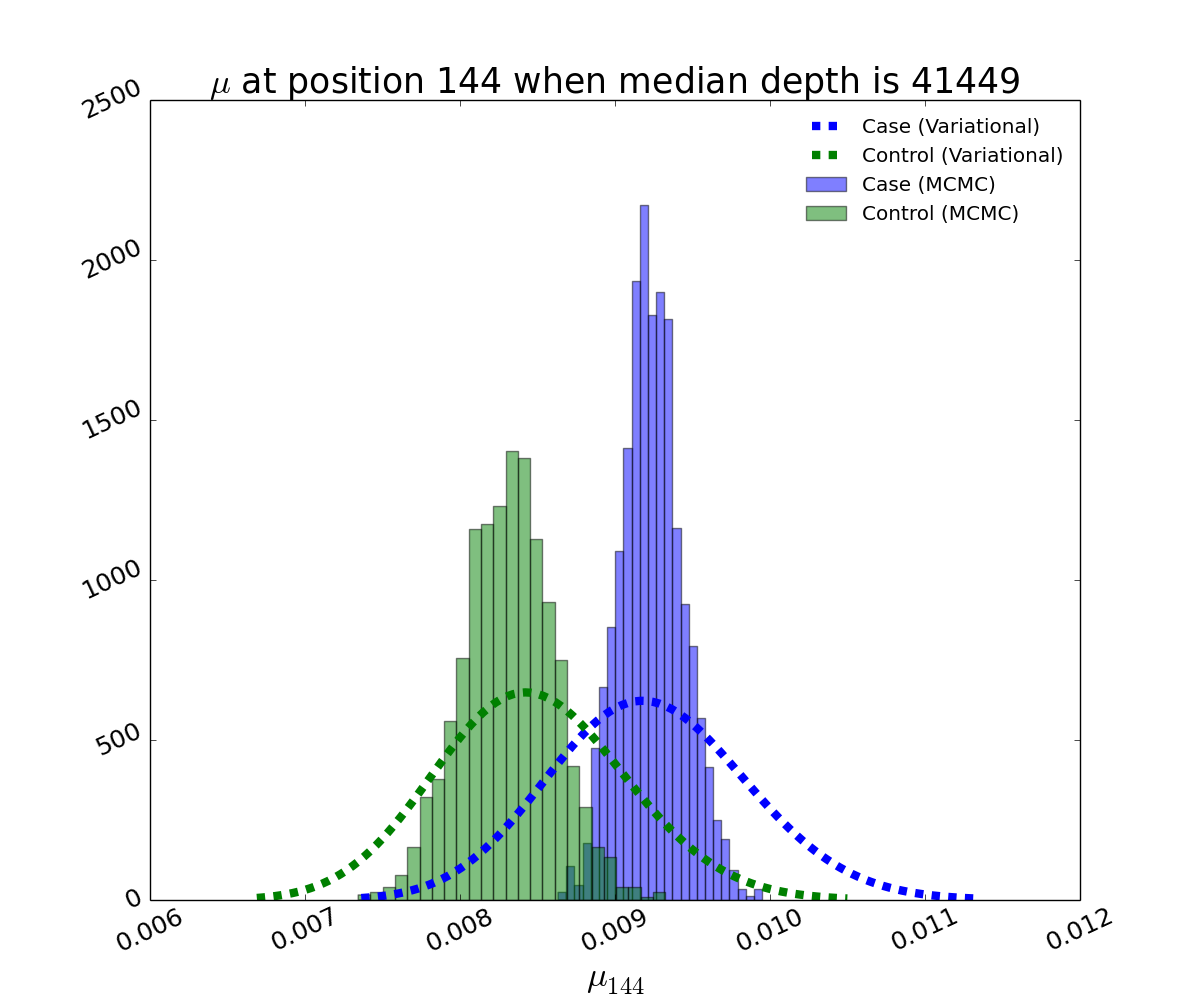
\includegraphics[width=0.4\textwidth]{figs/position_144_41449_mcmc_vs_var_mu.png}
%\caption{Approximated posterior distribution of position 144 when median read depth is 41449. This is a false positive position identified by MCMC, while variational algorithm does not identify this as a variant.}
%\vspace{-10pt}
%\label{tbl:posterior_mcmc_var_3}
%\end{figure}

\subsubsection*{Comparison of Timing}
Time for approximating variational posterior distribution is increased by increasing the length of region of interest and the median read depth (Figure~\ref{tbl:timing_mcmc_var}).
Variational algorithm works faster than MCMC at low read depths (27x and 298x), while MCMC works faster than variational algorithm at high read depths (3089x and 30590x).

% results are under folder \fzhang\Research\rvd3-variational-notebook\results\2015-10-15_Plot_time_vs_region_length_rvd3_synthetic_data
\begin{figure}[htbp]
\centering
%\vspace{-5pt}
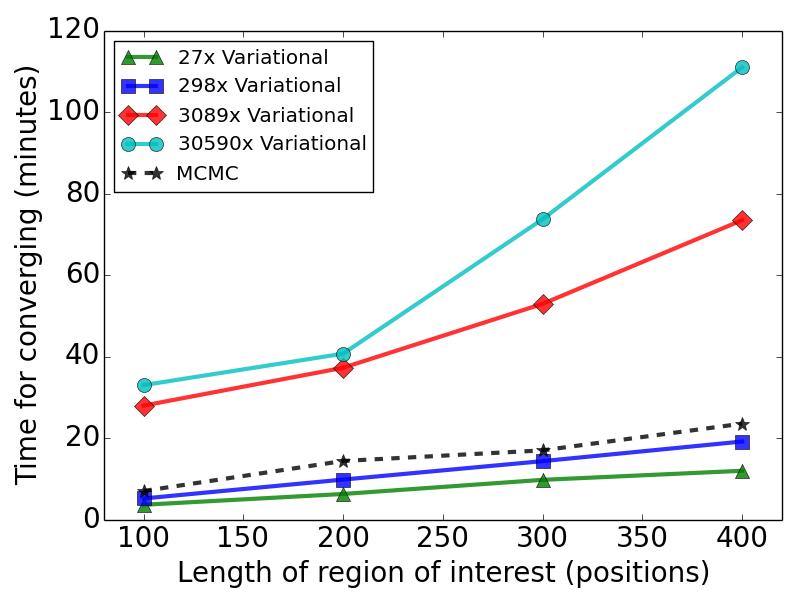
\includegraphics[width=0.5\textwidth]{tables/timing_var_mcmc.png}
\caption{Timing figure for variational algorithm and MCMC method.
60 processes are used to estimate the model on the synthetic data set.}
\vspace{-10pt}
\label{tbl:timing_mcmc_var}
\end{figure}

Timing profile for each parts of variational algorithm when median read depth is 3089x is also given in Figure~\ref{tbl:timing_profile_all}.
Optimizing $\gamma$ function in E-step and optimizing $M$ in M-step takes most of the time because an integration is needed.

% results are under folder \fzhang\Research\rvd3-variational-notebook\results\2015-10-21_Timing_profile_rvd3_program
\begin{figure*}{b}
\centering
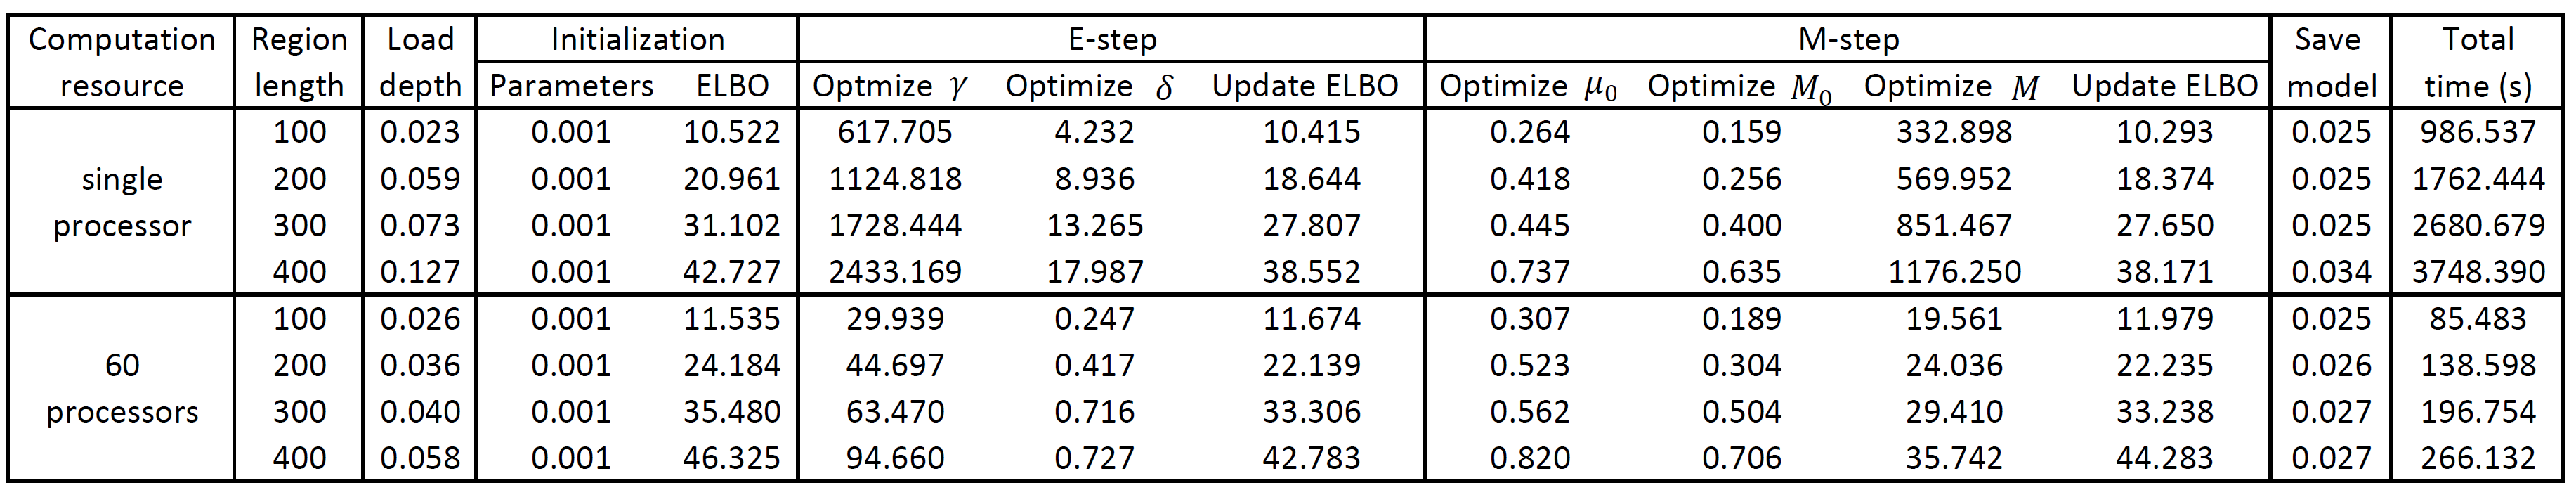
\includegraphics[width=1.0\textwidth]{tables/time_3089X_all.png}
\caption{Timing profile for one iteration of variational EM algorithm when median read depth is 3089x.
Single and multiple processors are both tested for timing to estimate the model on the synthetic data set.}
%\vspace{-10pt}
\label{tbl:timing_profile_all}
\end{figure*}

\subsection{Variants Detection on the Longitudinal Drug Resistance Data}
\subsubsection{Detected Drug Resistance Variants}
xxx\\
xxx\\
xxx\\
xxx\\
xxx\\
xxx\\
xxx\\


\subsubsection{Comparison to the State of Arts Approaches}
xxx\\
xxx\\
xxx\\
xxx\\
xxx\\
xxx\\
xxx\\
xxx\\
xxx\\
xxx\\
xxx\\
xxx\\
xxx\\
xxx\\
xxx\\
xxx\\

\subsection{Discussion}
1. Due to the absence of Bayesian conjugacy, we can also consider the Laplace approximation distribution as the proposal variational distribution for $\mu_j$.

2. How to improve the efficiency or our variational algorithm?

\section*{Acknowledgments}
Funding:


\appendix
%\section{Derivation of Variational Inference}

%% The file named.bst is a bibliography style file for BibTeX 0.99c
\bibliographystyle{named}
\bibliography{ijcai16}

\end{document}

